% Fig. 5 — Annotation efficiency curve (ILLUSTRATIVE placeholder data)
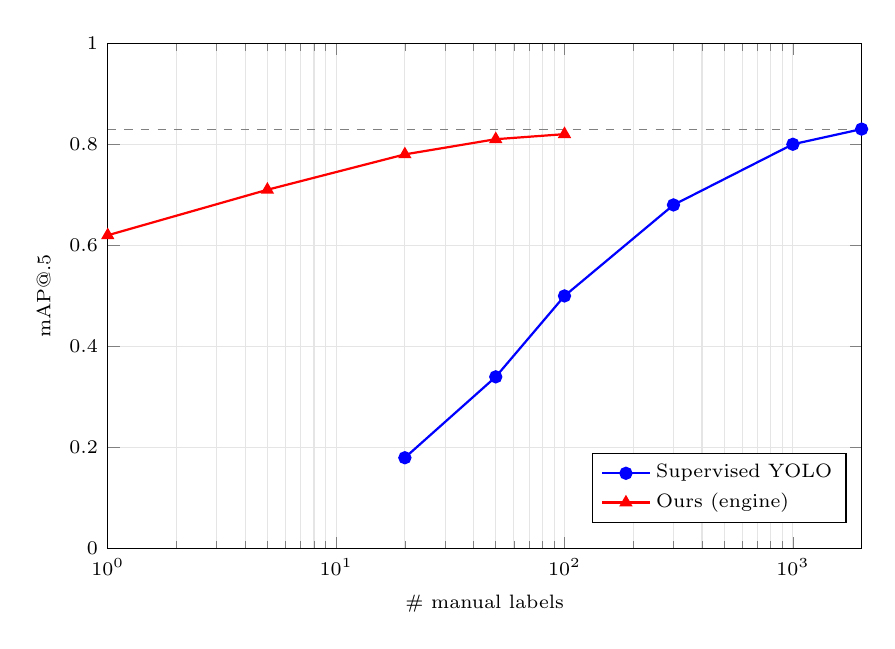
\begin{tikzpicture}
\begin{axis}[
  width=0.92\columnwidth, height=0.66\columnwidth,
  xlabel={\# manual labels}, ylabel={mAP@.5},
  xmode=log, log basis x=10,
  xmin=1, xmax=2000, ymin=0, ymax=1,
  grid=both, grid style={gray!20}, tick label style={font=\scriptsize},
  label style={font=\scriptsize},
  legend style={font=\scriptsize, at={(0.98,0.05)}, anchor=south east},
  legend cell align=left,
]
% supervised baseline (needs many labels) -- PLACEHOLDER
\addplot[mark=*, thick, blue] coordinates
  {(20,0.18)(50,0.34)(100,0.50)(300,0.68)(1000,0.80)(2000,0.83)};
\addlegendentry{Supervised YOLO}
% ours (auto-label, few/no manual) -- PLACEHOLDER
\addplot[mark=triangle*, thick, red] coordinates
  {(1,0.62)(5,0.71)(20,0.78)(50,0.81)(100,0.82)};
\addlegendentry{Ours (engine)}
% supervised plateau guide
\addplot[dashed, black!50, forget plot] coordinates {(1,0.83)(2000,0.83)};
\end{axis}
\end{tikzpicture}
